Os materiais utilizados para o experimento foram: goniômetro, lâmpadas de diferentes elementos químicos, lupa e prisma de numeração 17.

para  o início da coleta de dados, o primeiro passo se resumiu a calibrar o goniômetro. Para tal, o prisma foi retirado do goniômetro, a luneta de leitura foi destravada e alinhada com com a entrada de luz da lâmpada de Sódio, travando a luneta. Na sequência, o foco da luneta foi ajustado de para que a cruz no interior da mesma pudesse ser visto de forma nítida, assim como a fenda de entrada de luz; o parafuso de ajuste fino foi empregado para garantir que a cruz se alinhasse com o lado fixo da fenda. Para finalizar o ajuste, o disco graduado do goniômetro foi liberado seu "zero" foi alinhado com o "zero" da luneta.

Para próxima etapa do experimento, foi preciso determinar o ângulo $\alpha$ do ápice do prisma, isto é, a separação angular entre as duas faces do prisma mais próximas à fonte de luz. Para isto, considerou-se os dois raios luz $L_1$ e $L_2$ refletidos pelas faces do prisma, e o resultado geométrico que mostra que $\Delta \theta_L = \theta_{L_1} + \ang{360} - \theta_{L_2} = 2\alpha$, ou seja, a separação angular entre os raios é igual ao dobro do ápice, como ilustrado abaixo.

\begin{figure}[H]
	\centering	    
	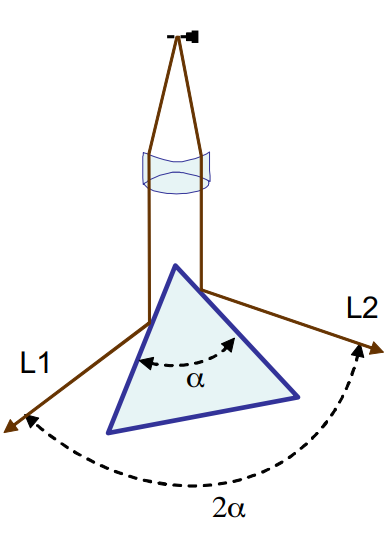
\includegraphics[scale=0.35]{figuras/alpha.png}
	\caption{Diagrama para a obtenção de $\alpha$}
	\label{fig:alpha}
\end{figure}

Com o ápice do prisma devidamente determinado, a fim de determinar o coeficientes $A$ e $B$ da equação de Cauchy:
\begin{equation}
    n(\lambda) = A + \frac{B}{\lambda^2}
    \label{eq:cauchy}
\end{equation}
Mostrando-se necessário coletar dados para o ângulo de desvio mínimo $\delta_\text{min}$ das raias espectrais de dispersão e determinar o índice de refração através da relação:

\begin{equation}
    n\left(\delta_\text{min}\right) = \frac{
        \sin\left(\frac{\alpha + \delta_\text{min}}{2}\right)
    }{
        \sin\left(\frac{\alpha}{2}\right)
    }
    \label{eq:n}
\end{equation}

 Assim, possibilitando a construção de um gráfico de $n$ por $1/\lambda^2$ em que $A$ e $B$ equivalem, respectivamente, aos coeficientes linear e angular do ajuste.

Para determinação dos desvios mínimos de cada raia espectral, lâmpadas baseadas em diferentes elementos químicos foram empregadas, no caso, os elementos utilizados foram: Sódio, Mercúrio, Cádmio e Hélio. O procedimento experimental consistia da observação das raias espectrais mais intensas geradas a partir da luz emitida pelas lâmpadas, de forma que o ângulo mínimo de dispersão de cada uma delas fosse medido com auxilio do goniômetro. Na sequência, os comprimentos de onda de cada raia foi obtido a partir de valores tabelados na literatura. Foram coletados dados para as 3 raias mais intensas de cada lâmpada, com exceção do Hélio, em que 4 raias puderam ser observadas com clareza.

Por fim, com os dados coletados, foi possível determinar os coeficiente $A$ e $B$ e por fim, utilizando a equação \ref{eq:n} e seguinte inversão da equação de Cauchy:
\begin{equation}
    \lambda = \sqrt{\frac{B}{n\left(\delta_\text{min}\right)-A}}
\end{equation}
foi gerada um curva que pode ser empregada como espectrômetro.


\subsection{Erros (só as fórmulas)}

O único tipo de medição experimental coletado diretamente foi o de ângulos, para os quais as resolução da medida era $\text{res}=\ang{;1;}$. Com base nisso, foram atríbuidas duas incertezas, a incerteza da leitura, que segue uma distribuição triangular de $\pm\text{res}/2$, e a incerteza de paralaxe do posicionamento na leitura, que poderia mover o encaixe dos minutos para as posições adjacentes, que foi calculada com uma distribuição retangular de $\pm\text{res}$. Por fim, a incerteza acumulada foi feita com base nas recomendações do GUM\cite{ref:gum}.

\begin{eqnarray}
    u_{\text{leitura}} = \frac{\text{res}}{2 \sqrt{6}} \\
    u_{\text{paralaxe}} = \frac{2\ \text{res}}{2 \sqrt{3}} \\
    \Delta{\delta_{\text{min}}} = \Delta\theta_L = u_{\text{medida}}
        = \sqrt{u_{\text{leitura}}^2 + u_{\text{paralaxe}}^2}
        = \frac{\text{res}}{2} \sqrt{\frac{3}{2}}
\end{eqnarray}

Todos os outros valores, calculados as partir desses ângulos e de valores referenciados de outros trabalhos, tiveram suas incertezas encontradas por meio da propagação das incertezas inicias, acompanhadas de inferências previstas por modelos estatísticos.

\begin{equation}
    \Delta{\alpha} = \sqrt{{\Delta{\text{L}_1}}^2\frac{1}{4} + {\Delta{\text{L}_2}}^2\frac{1}{4}} = \Delta\theta_L \frac{\sqrt{2}}{2}
\end{equation}

\begin{align}
    \Delta{n} &= \sqrt{
        \Delta{\alpha}^2 \left(\frac{\partial n}{\partial\alpha}\right)^2
        + \Delta{\delta^2_{\text{min}}} \left(\frac{\partial n}{\partial\delta_{\text{min}}}\right)^2
    } \\
    &= \frac{1}{2} \sqrt{
        \Delta{\alpha}^2 \frac{\sin^2(\delta_{\text{min}}/2)}{\sin^4({\alpha/2})}
        + \Delta{\delta^2_{\text{min}}} \frac{\cos(\alpha+\delta_{\text{min}})+1}{1-\cos(\alpha)}
    }
\end{align}

\begin{align}
    \Delta{\lambda} &= \sqrt{
        \Delta{A}^2 \left(\frac{\partial\lambda}{\partial A}\right)^2
        + \Delta{B}^2 \left(\frac{\partial\lambda}{\partial B}\right)^2
        + \Delta{\alpha}^2 \left(\frac{\partial\lambda}{\partial\alpha}\right)^2
        + \Delta{\delta^2_{\text{min}}} \left(\frac{\partial\lambda}{\partial \delta_{\text{min}}}\right)^2
    } \\
    &= \frac{1}{4 (n(\delta_{\text{min}})-A)} \sqrt{
        \Delta{A}^2\ 4 (\lambda(\delta_{\text{min}}))^2
        + \Delta{B}^2 \frac{4}{(\lambda(\delta_{\text{min}}))^2}
        + \Delta{\alpha}^2 (\lambda(\delta_{\text{min}}))^2 \frac{\sin^2(\delta_{\text{min}}/2)}{\sin^4(\alpha/2)}
        + \Delta{\delta^2_{\text{min}}} (\lambda(\delta_{\text{min}}))^2 \frac{\cos(\alpha+\delta_{\text{min}})+1}{1-\cos(\alpha)}
    }
\end{align}

No caso das incertezas de $A$ e $B$, o seu valor foi extraído pelo modelo de regressão linear por mínimos quadrados, como descrito no final do Guia de Incertezas~\cite{ref:gum}, bem como os valores utilizados para esses parâmetros.
